\documentclass[11pt,preprint, authoryear]{elsarticle}

\usepackage{lmodern}
%%%% My spacing
\usepackage{setspace}
\setstretch{1.2}
\DeclareMathSizes{12}{14}{10}{10}

% Wrap around which gives all figures included the [H] command, or places it "here". This can be tedious to code in Rmarkdown.
\usepackage{float}
\let\origfigure\figure
\let\endorigfigure\endfigure
\renewenvironment{figure}[1][2] {
    \expandafter\origfigure\expandafter[H]
} {
    \endorigfigure
}

\let\origtable\table
\let\endorigtable\endtable
\renewenvironment{table}[1][2] {
    \expandafter\origtable\expandafter[H]
} {
    \endorigtable
}


\usepackage{ifxetex,ifluatex}
\usepackage{fixltx2e} % provides \textsubscript
\ifnum 0\ifxetex 1\fi\ifluatex 1\fi=0 % if pdftex
  \usepackage[T1]{fontenc}
  \usepackage[utf8]{inputenc}
\else % if luatex or xelatex
  \ifxetex
    \usepackage{mathspec}
    \usepackage{xltxtra,xunicode}
  \else
    \usepackage{fontspec}
  \fi
  \defaultfontfeatures{Mapping=tex-text,Scale=MatchLowercase}
  \newcommand{\euro}{€}
\fi

\usepackage{amssymb, amsmath, amsthm, amsfonts}

\def\bibsection{\section*{References}} %%% Make "References" appear before bibliography


\usepackage[round]{natbib}

\usepackage{longtable}
\usepackage[margin=2.3cm,bottom=2cm,top=2.5cm, includefoot]{geometry}
\usepackage{fancyhdr}
\usepackage[bottom, hang, flushmargin]{footmisc}
\usepackage{graphicx}
\numberwithin{equation}{section}
\numberwithin{figure}{section}
\numberwithin{table}{section}
\setlength{\parindent}{0cm}
\setlength{\parskip}{1.3ex plus 0.5ex minus 0.3ex}
\usepackage{textcomp}
\renewcommand{\headrulewidth}{0.2pt}
\renewcommand{\footrulewidth}{0.3pt}

\usepackage{array}
\newcolumntype{x}[1]{>{\centering\arraybackslash\hspace{0pt}}p{#1}}

%%%%  Remove the "preprint submitted to" part. Don't worry about this either, it just looks better without it:
\makeatletter
\def\ps@pprintTitle{%
  \let\@oddhead\@empty
  \let\@evenhead\@empty
  \let\@oddfoot\@empty
  \let\@evenfoot\@oddfoot
}
\makeatother

 \def\tightlist{} % This allows for subbullets!

\usepackage{hyperref}
\hypersetup{breaklinks=true,
            bookmarks=true,
            colorlinks=true,
            citecolor=blue,
            urlcolor=blue,
            linkcolor=blue,
            pdfborder={0 0 0}}


% The following packages allow huxtable to work:
\usepackage{siunitx}
\usepackage{multirow}
\usepackage{hhline}
\usepackage{calc}
\usepackage{tabularx}
\usepackage{booktabs}
\usepackage{caption}


\newenvironment{columns}[1][]{}{}

\newenvironment{column}[1]{\begin{minipage}{#1}\ignorespaces}{%
\end{minipage}
\ifhmode\unskip\fi
\aftergroup\useignorespacesandallpars}

\def\useignorespacesandallpars#1\ignorespaces\fi{%
#1\fi\ignorespacesandallpars}

\makeatletter
\def\ignorespacesandallpars{%
  \@ifnextchar\par
    {\expandafter\ignorespacesandallpars\@gobble}%
    {}%
}
\makeatother

\newenvironment{CSLReferences}[2]{%
}

\urlstyle{same}  % don't use monospace font for urls
\setlength{\parindent}{0pt}
\setlength{\parskip}{6pt plus 2pt minus 1pt}
\setlength{\emergencystretch}{3em}  % prevent overfull lines
\setcounter{secnumdepth}{5}

%%% Use protect on footnotes to avoid problems with footnotes in titles
\let\rmarkdownfootnote\footnote%
\def\footnote{\protect\rmarkdownfootnote}
\IfFileExists{upquote.sty}{\usepackage{upquote}}{}

%%% Include extra packages specified by user

%%% Hard setting column skips for reports - this ensures greater consistency and control over the length settings in the document.
%% page layout
%% paragraphs
\setlength{\baselineskip}{12pt plus 0pt minus 0pt}
\setlength{\parskip}{12pt plus 0pt minus 0pt}
\setlength{\parindent}{0pt plus 0pt minus 0pt}
%% floats
\setlength{\floatsep}{12pt plus 0 pt minus 0pt}
\setlength{\textfloatsep}{20pt plus 0pt minus 0pt}
\setlength{\intextsep}{14pt plus 0pt minus 0pt}
\setlength{\dbltextfloatsep}{20pt plus 0pt minus 0pt}
\setlength{\dblfloatsep}{14pt plus 0pt minus 0pt}
%% maths
\setlength{\abovedisplayskip}{12pt plus 0pt minus 0pt}
\setlength{\belowdisplayskip}{12pt plus 0pt minus 0pt}
%% lists
\setlength{\topsep}{10pt plus 0pt minus 0pt}
\setlength{\partopsep}{3pt plus 0pt minus 0pt}
\setlength{\itemsep}{5pt plus 0pt minus 0pt}
\setlength{\labelsep}{8mm plus 0mm minus 0mm}
\setlength{\parsep}{\the\parskip}
\setlength{\listparindent}{\the\parindent}
%% verbatim
\setlength{\fboxsep}{5pt plus 0pt minus 0pt}



\begin{document}



\begin{frontmatter}  %

\title{Question 6: Portfolio Construction}

% Set to FALSE if wanting to remove title (for submission)




\author[Add1]{Austin Byrne}
\ead{}







\begin{abstract}
\small{
In this question I create optimal portfolios making use of Minimum
Variance Optimization. I first construct a unconstrained portfolio and
then compare it to the constrained portfolio. The constrained portfolio
results in lower risk and lower return.
}
\end{abstract}

\vspace{1cm}





\vspace{0.5cm}

\end{frontmatter}

\setcounter{footnote}{0}



%________________________
% Header and Footers
%%%%%%%%%%%%%%%%%%%%%%%%%%%%%%%%%
\pagestyle{fancy}
\chead{}
\rhead{}
\lfoot{}
\rfoot{\footnotesize Page \thepage}
\lhead{}
%\rfoot{\footnotesize Page \thepage } % "e.g. Page 2"
\cfoot{}

%\setlength\headheight{30pt}
%%%%%%%%%%%%%%%%%%%%%%%%%%%%%%%%%
%________________________

\headsep 35pt % So that header does not go over title




\hypertarget{introduction}{%
\section{\texorpdfstring{Introduction
\label{Introduction}}{Introduction }}\label{introduction}}

In this question I dive into the realm of portfolio construction. To
create an optimal portfolio I make use of the Minimum Variance Optimizer
(MVO) which creates an optimal portfolio with the lowest possible
variance. I construct an unconstrained and constrained portfolio using
MVO. The resulting optimal portfolios are low risk low return portfolios
which can be expected from using MVO. The constrained optimal portfolio
results in lower risk and lower annualized monthly returns.

\hypertarget{laod-relevant-functions}{%
\subsection{Laod relevant functions}\label{laod-relevant-functions}}

I load any function that I may have created so that I can use them in
this code and analysis.

\hypertarget{loading-relevant-data-and-packages}{%
\subsection{Loading relevant data and
packages}\label{loading-relevant-data-and-packages}}

Here I load the relevant data.

\hypertarget{data-preperation-lets-convert-the-price-data-to-monthly-returns-data}{%
\subsection{Data preperation: Lets convert the price data to monthly
returns
data}\label{data-preperation-lets-convert-the-price-data-to-monthly-returns-data}}

In this section I do some data perpetration. I take the original data of
the MAA and msci and create a new column called Monthly\_returns, which
calculates the monthly returns from the daily data. I also filter for
post 2010 and ensure that at least three years a data is available.

\hypertarget{maa-monthly-returns}{%
\subsubsection{MAA monthly returns}\label{maa-monthly-returns}}

Monthly returns for MAA are calculated after some fun wrangling.

\hypertarget{msci-monthly-returns}{%
\subsubsection{msci monthly returns}\label{msci-monthly-returns}}

Monthly returns for msci are calculated after some fun wrangling.

\hypertarget{creating-an-asset-class-column-in-my-data-sets}{%
\subsubsection{Creating an asset class column in my data
sets}\label{creating-an-asset-class-column-in-my-data-sets}}

There are now four different asset classes in the MAA data set, namely,
``Assian currency'', ``Credit'', ``Rates'', ``Commodity'', ``Equity'',
and ``Real estate.

\hypertarget{lets-now-attempt-to-construct-the-portfolio-by-making-use-of-mean-variance-optimization}{%
\subsection{Lets now attempt to construct the portfolio by making use of
mean variance
optimization:}\label{lets-now-attempt-to-construct-the-portfolio-by-making-use-of-mean-variance-optimization}}

I now make use of ean VAriance Optimization to first create a
unconstrained portfolio. I am then able to evaluate the risk and return
of the unconstrained portfolio which I then compare to the constrained
portfolio.

\hypertarget{combine-the-data-sets-and-compute-some-graphs}{%
\subsubsection{Combine the Data Sets and compute some
graphs}\label{combine-the-data-sets-and-compute-some-graphs}}

Here I make use of a function I created that prepares and combines the
relavant data.

\hypertarget{rolling-3-year-annualzied-returns-comparison-of-asset-classes}{%
\subsubsection{Rolling 3 year annualzied returns comparison of asset
classes}\label{rolling-3-year-annualzied-returns-comparison-of-asset-classes}}

TO insoect the data in question I run a plot that conatins the 3 year
annualsied returns for each asset class. What is immidatley evident in
this plot is that the equities asset class is the most volatile which
also means the asset class that potentially holds the most risk. Outside
of the equities asset class, the remaining asset classes are relatively
similiar, with USD beinf the next most volatile.

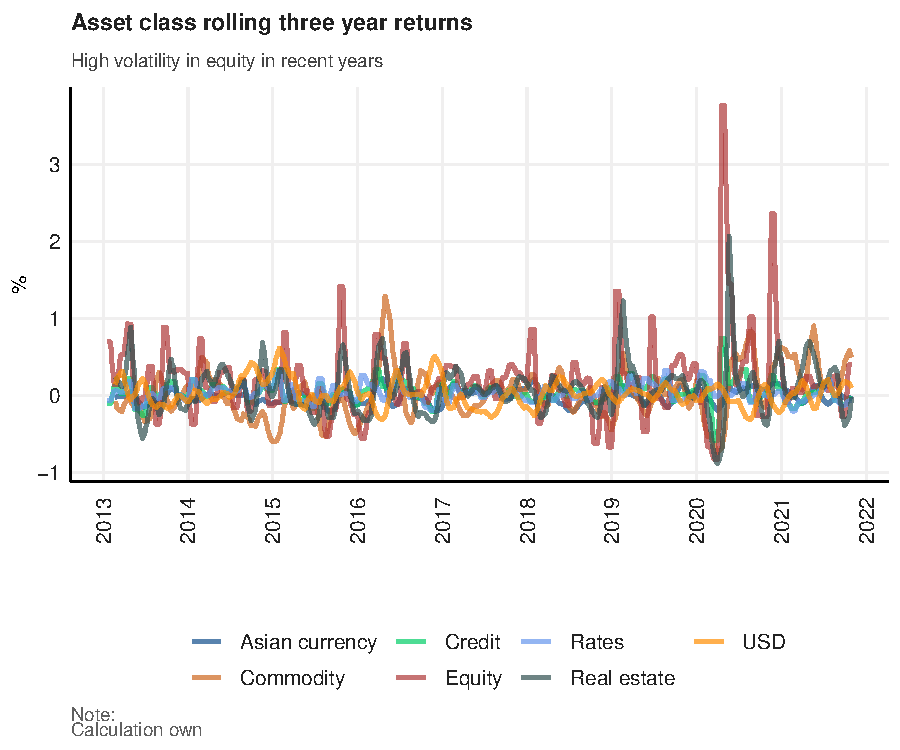
\includegraphics{Question-6_files/figure-latex/unnamed-chunk-7-1.pdf}

\hypertarget{boxplot-of-monthly-returns-by-asset-class}{%
\subsubsection{Boxplot of monthly returns by Asset
class}\label{boxplot-of-monthly-returns-by-asset-class}}

Here I make use of a function I create to obtain the boxplot for each
asset class which illustrates the distribution of monthly returns for
each asset class. The equity asset class as expected has the highest
average monthly return but also contains alot of outliers which can be
expected after seeing how volatile the returns of equity can be. The
most stable asset classes seem to be the Asian currency and USD. This
plot creates a nice illustration of the spread of monthly returns for
each asset class.

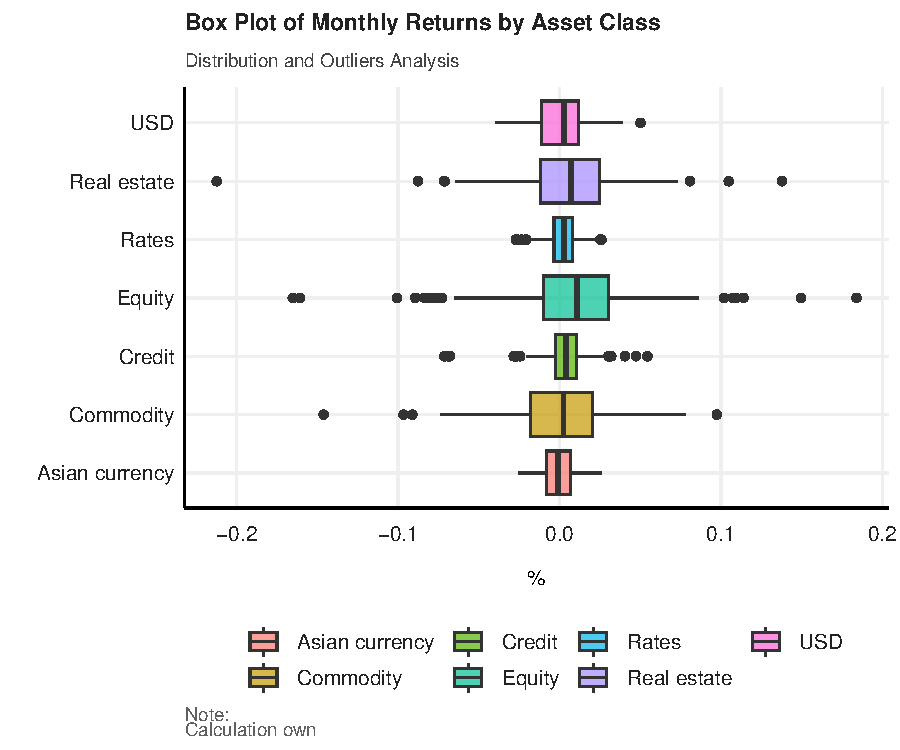
\includegraphics{Question-6_files/figure-latex/unnamed-chunk-8-1.pdf}

\hypertarget{computing-the-returns-matrix}{%
\subsubsection{Computing the returns
matrix}\label{computing-the-returns-matrix}}

In order to using the Minimum Variance Optimizer I need to first craete
a returns matrix, whicg contains the returns of each asset class in a
matrix. TO do this I make use of a function that was crated in the
practical.

\hypertarget{computing-the-simple-covariance-matrix}{%
\subsubsection{Computing the simple covariance
matrix}\label{computing-the-simple-covariance-matrix}}

Like that of the returns matrix one needs to create a simple covariance
matrix to make use of MVO and be able to create an optimal portfolio.

\hypertarget{using-minimum-variance-optimization-mvo-for-an-unrestricted-portfolio.}{%
\subsubsection{Using Minimum variance optimization (MVO) for an
unrestricted
portfolio.}\label{using-minimum-variance-optimization-mvo-for-an-unrestricted-portfolio.}}

Now using MVO I am able to construct an unconstrained optimal portfolio
and evaluate the risk and returns. The risk will be evaluated by the
standard deviation.

As can be seen from the table below, The optimal unconstrained portfolio
has a standard deviation of 0.09827125 and an average annualized monthly
retun of 0.02648242. Thus the portfolio has a very low standard
deviation which is expected since the portfolio was constructed using
MVO. Since the portfolio takes on low risk, it is not suprising to see
that the return is also fairly low at 0.02648242. Thus, the
unconstrained optimal portfolio using MVO is a low risk low return
portfolio.

Lets now add the constraints in and then compare to this base portfolio.

\begin{verbatim}
## # A tibble: 1 x 2
##   average_ret_Ann volatility_Ann
##             <dbl>          <dbl>
## 1          0.0265         0.0983
\end{verbatim}

\hypertarget{now-lets-create-the-constrained-optimised-portfolio}{%
\subsubsection{Now lets create the constrained optimised
portfolio}\label{now-lets-create-the-constrained-optimised-portfolio}}

With the specific constraints being: Apply Quarterly Rebalancing; -
Limit exposure to Bonds and credit instruments at 25\%; - Limit exposure
to Equities at 60\%; - Limit single asset exposure at 40\%

\hypertarget{lets-first-create-some-bondcredit-and-equity-idicies-that-we-can-use-for-our-constraints-later}{%
\paragraph{Lets first create some bond/credit and equity idicies that we
can use for our constraints
later}\label{lets-first-create-some-bondcredit-and-equity-idicies-that-we-can-use-for-our-constraints-later}}

Here I create the constraints that will be used to construct the
constrained optimal portfolio.

\#Adding constraints to the optimisation problem and solving

Solving for the constrained optimal portfolio is done using the CVXR
package in R.

Lets now evaluate the constrained portfolio. The constrained optimal
portfolio is an even lower risk and lower retun portfolio than that of
the unconstrained portfolio created previously. The standard deviation
is now at 0.0003147487 and the monthly annualised return is at
0.0003147487. Thus by adding the constrains to the portfolio we decrease
the risk in the portfolio through decreased standard deviation, however,
with decreased risk come decreased returns. Once again since we make use
of MVO to create the optimal portfolio, it is not surprising that the
optimal portfolio is a low risk low return optimal portfolio.

\begin{verbatim}
##       [,1]
##  [1,] 0.01
##  [2,] 0.01
##  [3,] 0.01
##  [4,] 0.01
##  [5,] 0.01
##  [6,] 0.27
##  [7,] 0.01
##  [8,] 0.40
##  [9,] 0.01
## [10,] 0.01
## [11,] 0.01
## [12,] 0.01
## [13,] 0.23
\end{verbatim}

\begin{verbatim}
## # A tibble: 13 x 2
##    stocks         weight
##    <chr>           <dbl>
##  1 ADXY Index       0.01
##  2 BCOMTR Index     0.01
##  3 DXY Index        0.01
##  4 LEATTREU Index   0.01
##  5 LGAGTRUH Index   0.01
##  6 LGCPTRUH Index   0.27
##  7 LP05TREH Index   0.01
##  8 LUACTRUU Index   0.4 
##  9 LUAGTRUU Index   0.01
## 10 MSCI_ACWI        0.01
## 11 MSCI_Jap         0.01
## 12 MSCI_RE          0.01
## 13 MSCI_USA         0.23
\end{verbatim}

\begin{verbatim}
## [1] 0.0003147487
\end{verbatim}

\begin{verbatim}
## [1] 0.005250953
\end{verbatim}

\begin{longtable}[]{@{}lr@{}}
\caption{Portfolio Performance Metrics}\tabularnewline
\toprule\noalign{}
Metric & Value \\
\midrule\noalign{}
\endfirsthead
\toprule\noalign{}
Metric & Value \\
\midrule\noalign{}
\endhead
\bottomrule\noalign{}
\endlastfoot
Annualized Return & 0.0052510 \\
Annualized Risk & 0.0003147 \\
\end{longtable}

\newpage

\hypertarget{references}{%
\section*{References}\label{references}}
\addcontentsline{toc}{section}{References}

\hypertarget{refs}{}
\begin{CSLReferences}{0}{0}
\end{CSLReferences}

\hypertarget{appendix}{%
\section*{Appendix}\label{appendix}}
\addcontentsline{toc}{section}{Appendix}

\hypertarget{appendix-a}{%
\subsection*{Appendix A}\label{appendix-a}}
\addcontentsline{toc}{subsection}{Appendix A}

Some appendix information here

\hypertarget{appendix-b}{%
\subsection*{Appendix B}\label{appendix-b}}
\addcontentsline{toc}{subsection}{Appendix B}

\bibliography{Tex/ref}





\end{document}
